\chapter{Implementation, Engineering\\Post-Mortem, and Safety}
\label{ch:impl_postmortem}

\section{Full-Stack System Implementation}
To provide production-grade operability, the platform is implemented as a full-stack distributed system combining asynchronous Python microservices with a modern React 18 TypeScript web console.

\subsection{FastAPI Backend and WebSocket Streaming}
The backend service (\texttt{future/api/main.py}) runs on Uvicorn with an asynchronous event loop listening on port 8000. It mediates between the Ryu controller, the LangGraph agent, and connected frontend web clients.
\begin{itemize}[noitemsep,topsep=2pt]
  \item \textbf{WebSocket Real-Time Stream (\texttt{/ws/telemetry})}: Broadcasts telemetry snapshots every 500\,ms (2\,Hz), packaging link rates, port dropped packet counts, bottleneck status, and ML hazard probabilities into a lightweight JSON payload.
  \item \textbf{Thread-Safe Global State}: Communication between Ryu's Eventlet greenlet loop and FastAPI's asyncio loop uses atomic thread locks to synchronize routing mode, active topology, and verify engine verdicts.
\end{itemize}

\subsection{React 18 Interactive Console and Topologies Canvas}
The frontend console (\texttt{future/dashboard/react-app}) is a single-page application built with React 18, TypeScript, and Vite.
\begin{itemize}[noitemsep,topsep=2pt]
  \item \textbf{Dynamic Canvas Visualizer}: Renders switches, hosts, and interconnecting links via scalable vector graphics (SVG) across three projection modes: 2D Blueprint, 3D Perspective Isometric, and 3D Topdown Plan.
  \item \textbf{LangGraph Agent Modal}: An interactive modal (\texttt{AgentModal.tsx}) supporting natural-language chat and one-click action pills: \texttt{[Create Congestion]}, \texttt{[Fix Congestion]}, and \texttt{[Audit Telemetry]}. The modal displays an execution pipeline trace showing live checkmarks across the five stages (\textit{Monitor} $\to$ \textit{Analyze} $\to$ \textit{Plan} $\to$ \textit{Act} $\to$ \textit{Verify}) with execution timestamps.
  \item \textbf{Empirical Markdown Viewer}: A dedicated React component (\texttt{MarkdownReportView.tsx}) parsing raw Markdown from \texttt{results/RESULTS.md} into monospace statistical tables with sticky headers, verdict badges (\texttt{Best Observed}, \texttt{Separated (p < 0.05)}, \texttt{Overlapping 95\% CI}), provenance alerts, and Copy/Download Markdown controls.
\end{itemize}

\begin{figure}[H]
  \centering
  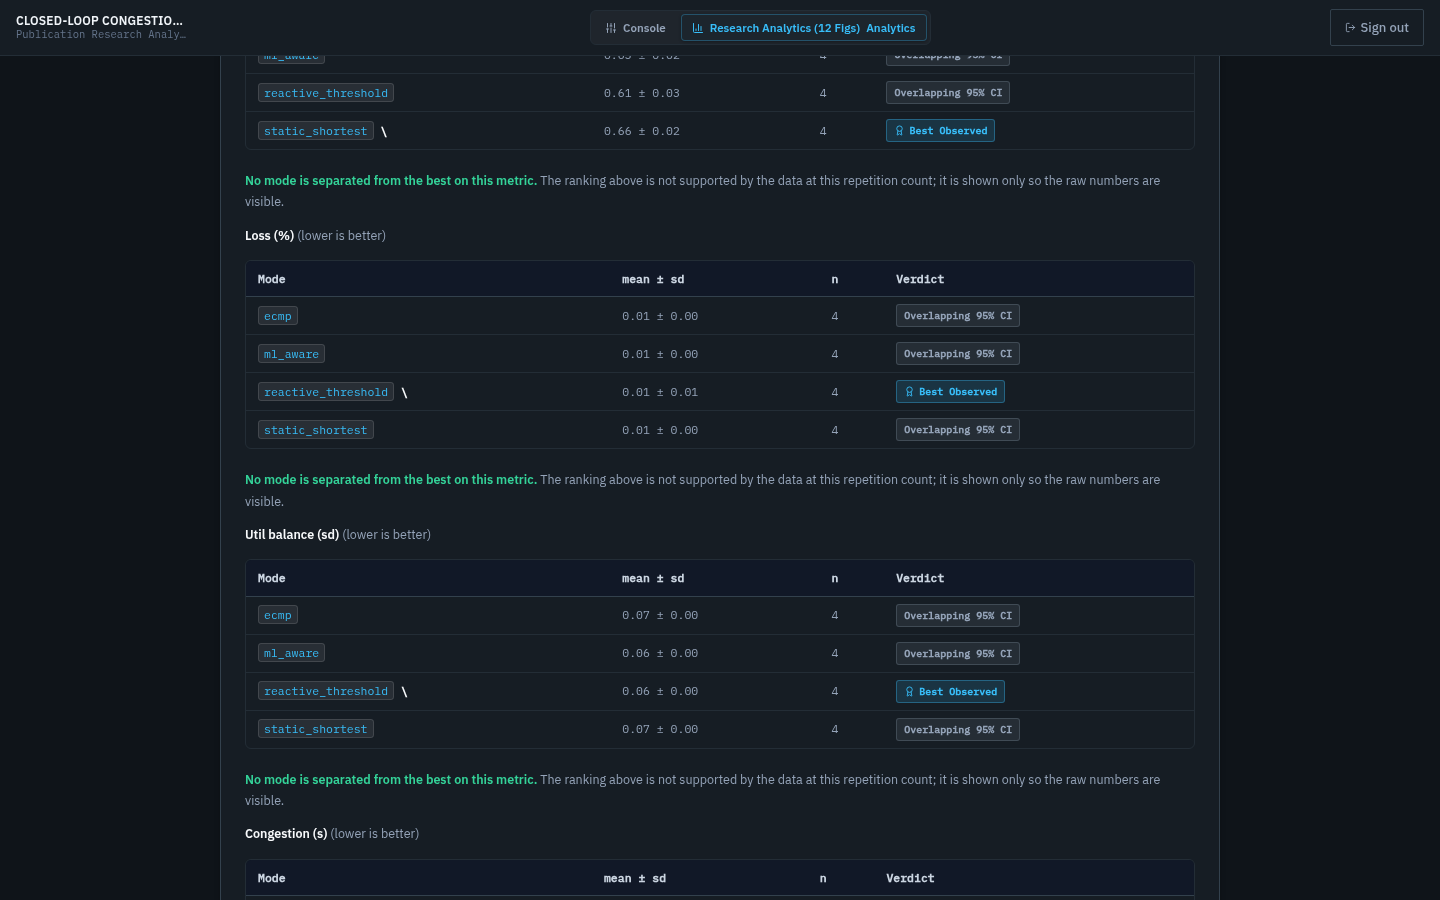
\includegraphics[width=0.68\textwidth]{analytics_markdown_report_tab.png}
  \caption{Empirical Markdown Report viewer rendered in the frontend console, presenting statistical hypothesis tests and non-overlapping confidence intervals.}
  \label{fig:ui_markdown_report_ch6}
\end{figure}

\section{Engineering Post-Mortem: Diagnostic Rigor}
In experimental systems research, software defects rarely manifest as clean, loud exceptions. More often, they present as silent statistical distortions. Rather than adjusting hyper-parameters to mask unexpected outputs, every discrepancy encountered was diagnosed to root cause, solved at the architectural level, and guarded with automated mutation tests.

\subsection{1. The Silent Controller Pipe-Buffer Deadlock}
\textbf{Symptom}: During initial 90-second collection sweeps, telemetry output ceased abruptly approximately 24 seconds into every run. The collector emitted exactly 13 samples per link instead of the expected 45--47 samples. The controller was alive, but completely inert.

\textbf{Root Cause}: Ryu was spawned via \texttt{subprocess.Popen} with \texttt{stdout=subprocess.PIPE} with nothing draining the pipe. In Linux, an anonymous pipe buffer is finite (64\,KiB). Once cumulative OpenFlow event logs exceeded 64\,KiB at $\sim$24\,s, Ryu's \texttt{sys.stdout.write()} blocked inside the Linux kernel. Because Ryu runs on Eventlet cooperative greenlets within a single OS process, blocking in a C-level write halted the greenlet event loop, freezing all network telemetry collection.

\textbf{Architectural Fix}: The fix replaces pipe buffers with non-blocking file descriptor redirection using a dedicated \texttt{ControllerLog} context manager writing directly to disk files. A file descriptor never applies back-pressure to the writing process, preventing kernel deadlock. Telemetry capture expanded from \textbf{24 seconds to 92 seconds}, and samples per link increased from \textbf{13 to 47}.

\subsection{2. Duplicate Port-Stats Telemetry Measurements}
\textbf{Symptom}: During model training, pandas raised an exception during time-series indexing: \texttt{ValueError: series has 1 duplicate timestamp(s)}.

\textbf{Root Cause}: Telemetry timestamps come from the switch's OpenFlow port-stats reply header (\texttt{duration\_sec}, \texttt{duration\_nsec}). When an asynchronous OpenFlow reply was delayed due to control-plane congestion, the fixed 2.0-second timer timed out and wrote the previous sample's cached values. When the delayed reply arrived, the collector wrote it with the identical switch timestamp, creating duplicate measurements.

\textbf{Architectural Fix}: An atomic \textbf{watermark gate} was installed in the collector. If a sample's timestamp does not strictly exceed the previous recorded timestamp for that link ($t \le t_{\text{prev}}$), the write is suppressed.

\subsection{3. Traffic Generator Fragility: Process Spawning vs. Kernel TC}
\textbf{Symptom}: Link utilization profiles for the \texttt{ramp} pattern did not exhibit a continuous stair-step progression. Instead, the link transitioned abruptly from 0\,Mbps to 10\,Mbps inside a single 2-second interval, mimicking a square wave.

\textbf{Root Cause}: \texttt{traffic/generate.py} spawned an individual \texttt{iperf3} process for each ramp step via Mininet's \texttt{node.cmd()}. Mininet's \texttt{cmd()} incurs hundreds of milliseconds of pty allocation overhead, causing steps to be skipped. Furthermore, when an \texttt{iperf3} process reached its declared $-t$ duration, it exited; if the subsequent command was delayed by even 50\,ms, interface traffic collapsed to zero between steps.

\textbf{Architectural Fix}: We decoupled traffic generation from process scheduling. We start \textbf{a single, long-lived \texttt{iperf3} client} offering maximum rate, and use the Linux kernel Traffic Control Token Bucket Filter (\texttt{tc qdisc change dev eth1 root tbf rate ...}) to shape egress rate dynamically. Because \texttt{tc} commands execute synchronously inside the kernel in sub-millisecond time, step transitions are instantaneous, continuous, and immune to process teardown.

\subsection{4. Substring Intent Collision in Agent Chat Router}
\textbf{Symptom}: Prompting the agent with \textit{``fix the congestion''} caused the backend to trigger \texttt{inject\_congestion()} rather than \texttt{run\_mitigation()}.

\textbf{Root Cause}: A naive substring check in the FastAPI router checked \texttt{"congest" in msg.lower()}. Because \textit{congestion} contains \textit{congest}, the mitigation request matched the injection branch.

\textbf{Architectural Fix}: The router was refactored with priority-ordered keyword matching, checking explicit mitigation keywords first (\texttt{fix}, \texttt{mitigate}, \texttt{reroute}, \texttt{detour}) before checking injection phrases.

\subsection{5. Canvas SVG Line Z-Index Bleed-Through}
\textbf{Symptom}: When the agent modal was opened, SVG link paths and animated traffic particles from the background canvas remained clickable and visually bled through the modal backdrop.

\textbf{Architectural Fix}: Explicit global CSS stacking tokens were assigned, raising \texttt{.modal-backdrop} to \texttt{z-index: 99999}, completely isolating the modal over all canvas SVG layers.

\section{Operational Safety and Scalability Bounds}

\subsection{TCAM Memory Bounds}
To prevent switch Ternary Content-Addressable Memory (TCAM) exhaustion, the controller uses hierarchical wildcard prefix aggregation rather than per-flow rules:
\begin{equation}
  N_{\text{TCAM}} = \mathcal{O}(|P_{\text{detour}}|) \quad \text{instead of} \quad \mathcal{O}(|\text{Flows}| \cdot |P_{\text{detour}}|)
\end{equation}
On the 9-city Abilene WAN backbone, activating a 5-hop detour requires installing exactly \textbf{5 flow entries} across the fabric, consuming less than $0.1\%$ of available switch TCAM capacity.

\subsection{Route Flapping and Hysteresis Cooldown}
To prevent traffic from perpetually bouncing between primary and detour links, the decision engine enforces a three-tier hysteresis filter:
\begin{enumerate}[noitemsep,topsep=2pt]
  \item \textbf{Dwell Time ($T_{\text{dwell}} = 10$\,s)}: Once a detour path is installed, it remains locked for a minimum dwell duration.
  \item \textbf{Cooldown Timer ($T_{\text{cooldown}} = 15$\,s)}: Following any reroute or rollback event, subsequent routing modifications are prohibited for 15 seconds.
  \item \textbf{Improvement Ratio Threshold ($\Delta_{\text{thresh}} = 1.25$)}: An alternate path is selected only if its calculated cost represents at least a 25\% improvement over the current path.
\end{enumerate}
All installed detour flow entries carry an OpenFlow \texttt{hard\_timeout = 60} seconds, ensuring that in the event of total controller failure, rules automatically age out in switch hardware, restoring static baseline forwarding.
